\section{Strategy 4: Tensor Extension with Declared Losses}

\subsection{Method}

We designed a fourth evaluation strategy (S4) that extends S1 by
requiring the model to declare \textbf{structured losses} alongside its
T/I/F values. Each loss is a triple:

\begin{itemize}
\tightlist
\item
  \textbf{what}: What the model cannot evaluate (brief description)
\item
  \textbf{why}: Why this limits the assessment
\item
  \textbf{severity}: Impact on the evaluation {[}0.0 to 1.0{]}
\end{itemize}

The prompt explicitly requires at least one declared loss and states
that ``honesty about limits is required.'' Full prompt text in Appendix
A.

We ran S4 across all 5 models, 5 phenomena, and 5 repetitions (125
evaluations) with max\_tokens=500. This proved insufficient for
Mistral's verbose loss declarations, causing 18 parse failures from
truncated JSON. Mistral was re-run at max\_tokens=1500, producing 25
complete evaluations with 0 parse failures. The Mistral results reported
below use the 1500-token rerun data exclusively.

\subsection{The Key Test: Do Losses Differentiate What Scalars Cannot?}

For each model, we computed two metrics comparing paradox vs.~ignorance:

\begin{enumerate}
\def\labelenumi{\arabic{enumi}.}
\tightlist
\item
  \textbf{Scalar Manhattan distance}: \textbar T\_p - T\_i\textbar{} +
  \textbar I\_p - I\_i\textbar{} + \textbar F\_p - F\_i\textbar{} where
  p = paradox, i = ignorance
\item
  \textbf{Loss vocabulary Jaccard similarity}: Word-level token overlap
  between the ``what'' fields of declared losses for the two phenomena
  (the concise loss description, not the explanatory ``why'' field)
\end{enumerate}

\begin{longtable}[]{@{}
  >{\raggedright\arraybackslash}p{(\columnwidth - 6\tabcolsep) * \real{0.3182}}
  >{\centering\arraybackslash}p{(\columnwidth - 6\tabcolsep) * \real{0.1364}}
  >{\centering\arraybackslash}p{(\columnwidth - 6\tabcolsep) * \real{0.1364}}
  >{\raggedright\arraybackslash}p{(\columnwidth - 6\tabcolsep) * \real{0.4091}}@{}}
\toprule\noalign{}
\begin{minipage}[b]{\linewidth}\raggedright
Model
\end{minipage} & \begin{minipage}[b]{\linewidth}\centering
Scalar Distance
\end{minipage} & \begin{minipage}[b]{\linewidth}\centering
Loss Jaccard
\end{minipage} & \begin{minipage}[b]{\linewidth}\raggedright
Finding
\end{minipage} \\
\midrule\noalign{}
\endhead
\bottomrule\noalign{}
\endlastfoot
Claude Sonnet 4.6 & 0.034 & 0.097 & Scalars barely distinguish; losses
fully distinguish \\
DeepSeek V3 & 0.540 & 0.083 & Both channels distinguish \\
Llama 4 Maverick & 0.040 & 0.056 & Scalars nearly identical; losses
disjoint \\
Mistral Medium 3.1 & \textbf{0.000} & \textbf{0.066} & \textbf{Scalars
identical; losses completely different} \\
Qwen3-235B & 0.340 & 0.070 & Both channels distinguish \\
\end{longtable}

\textbf{Every model produces nearly disjoint loss vocabularies} for
paradox vs.~ignorance (Jaccard < 0.10), regardless of whether
the scalars distinguish the phenomena. The maximum vocabulary overlap is
9.7\% (Claude). The minimum is 5.6\% (Llama).

\begin{figure}
\centering
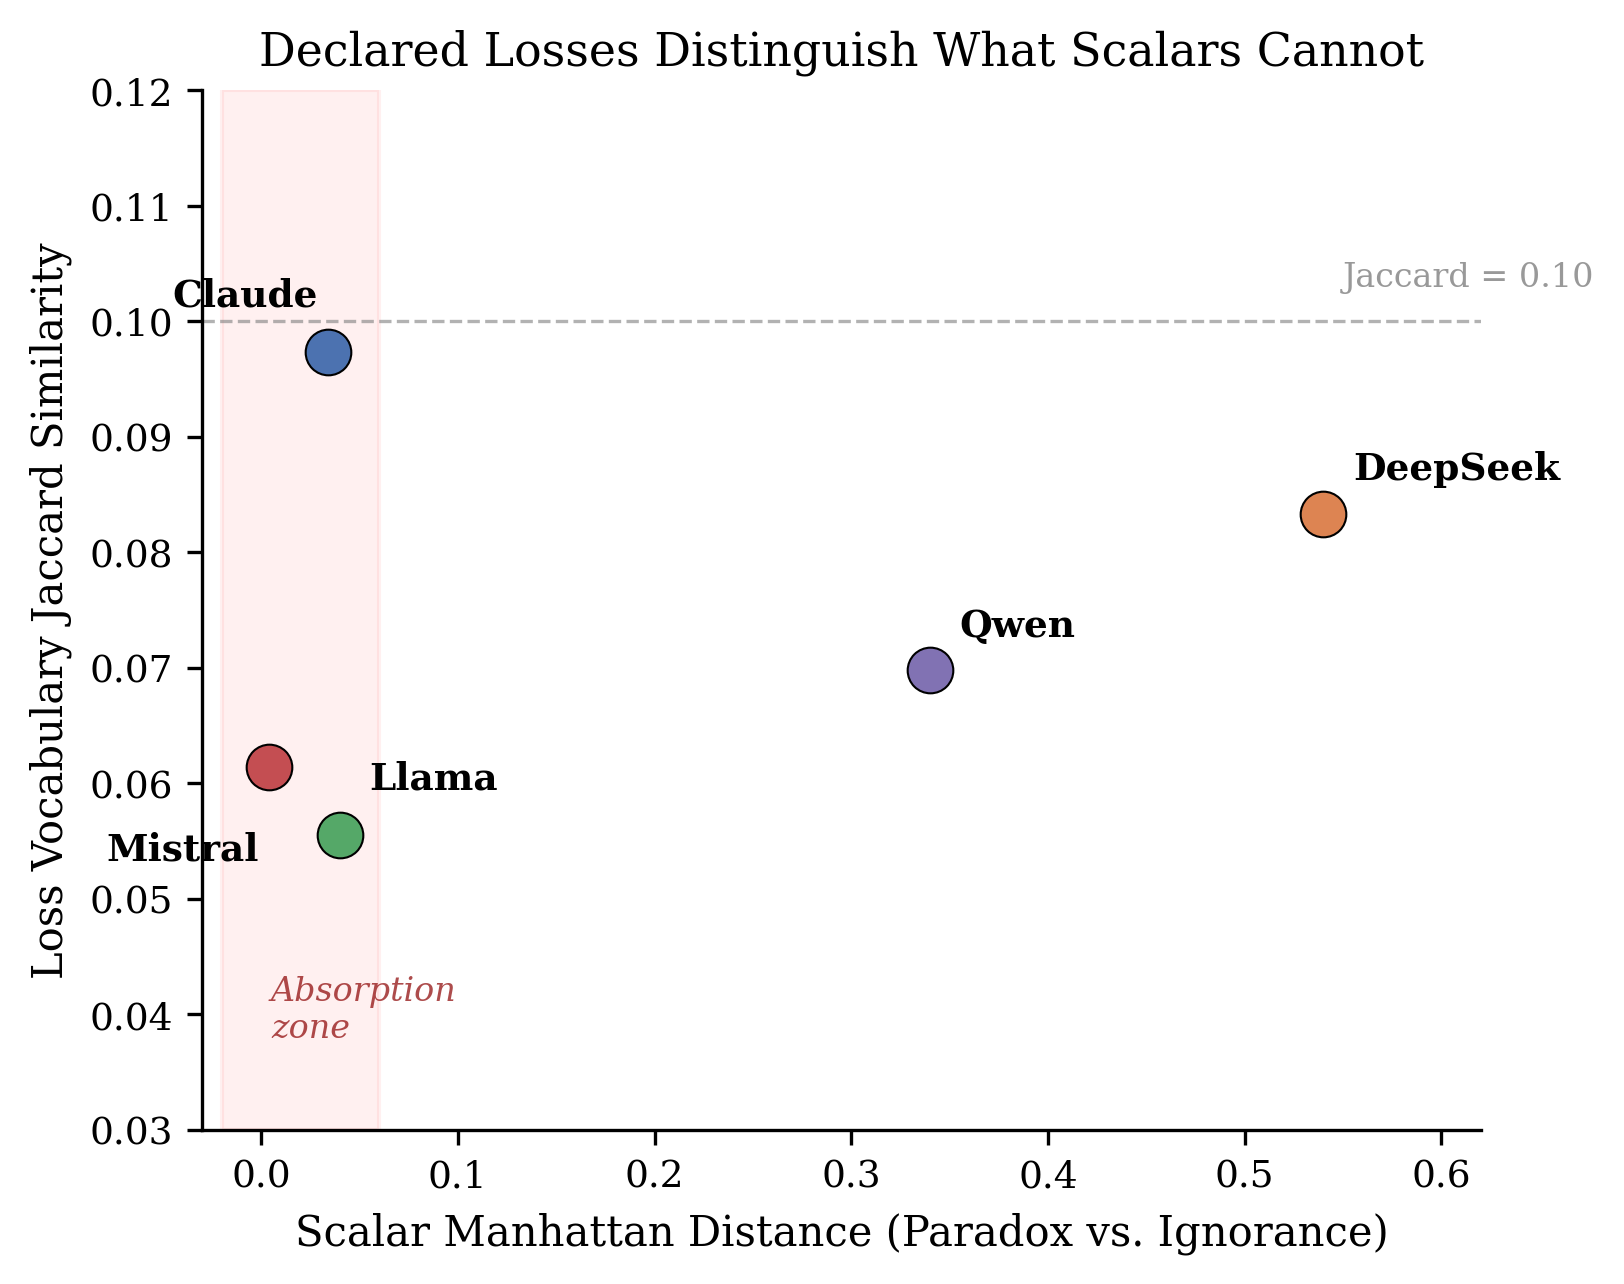
\includegraphics{fig_scalar_vs_jaccard.png}
\caption{Figure 2: Scalar distance vs.~loss Jaccard similarity}
\end{figure}

\emph{Figure 2: Scalar Manhattan distance (x-axis) vs.~loss vocabulary
Jaccard similarity (y-axis) for paradox vs.~ignorance across five
models. Models in the Absorption zone (red shading) produce near-zero
scalar differences yet completely different loss declarations. All
models fall below Jaccard = 0.10.}

\subsection{Mistral: The Critical Case}

Mistral is the strongest test because it predominantly exhibits
Absorption by producing (T=0, I=1, F=0) as its modal response for both
paradox and ignorance in S1 and S4:

\textbf{S4 Paradox} (T=0.0, I=1.0, F=0.0): ``Self-referential paradox
resolution'' (severity 1.0), ``Formal system dependency'' (0.8),
``Contextual grounding of `this sentence'\,'' (1.0)

\textbf{S4 Ignorance} (T=0.0, I=1.0, F=0.0): ``Empirical unknowability
of the exact number of stars'' (severity 1.0), ``Definition of
`universe' in cosmological context'' (0.9), ``Mathematical ambiguity of
`even' for infinite quantities'' (0.8)

The scalars are identical. The losses are domain-specific, accurate, and
completely different. The model \textbf{has} the internal distinction:
the scalar output format cannot express it.

\subsection{Pairwise Loss Differentiation (Mistral)}

The full pairwise Jaccard matrix for Mistral across all five phenomena
(from the 1500-token rerun, 25 evaluations, 0 parse failures):

\begin{longtable}[]{@{}llllll@{}}
\toprule\noalign{}
& Par & Ign & Vag & Con & Fut \\
\midrule\noalign{}
\endhead
\bottomrule\noalign{}
\endlastfoot
\textbf{Paradox} & 1.000 & 0.061 & 0.089 & 0.126 & 0.074 \\
\textbf{Ignorance} & & 1.000 & 0.089 & 0.116 & 0.084 \\
\textbf{Vagueness} & & & 1.000 & 0.143 & 0.091 \\
\textbf{Contradiction} & & & & 1.000 & 0.099 \\
\textbf{Contingency} & & & & & 1.000 \\
\end{longtable}

Every off-diagonal cell is below 0.15. Five phenomena, five nearly
disjoint loss vocabularies from a model that produces nearly identical
scalars for three of them.

\begin{figure}
\centering
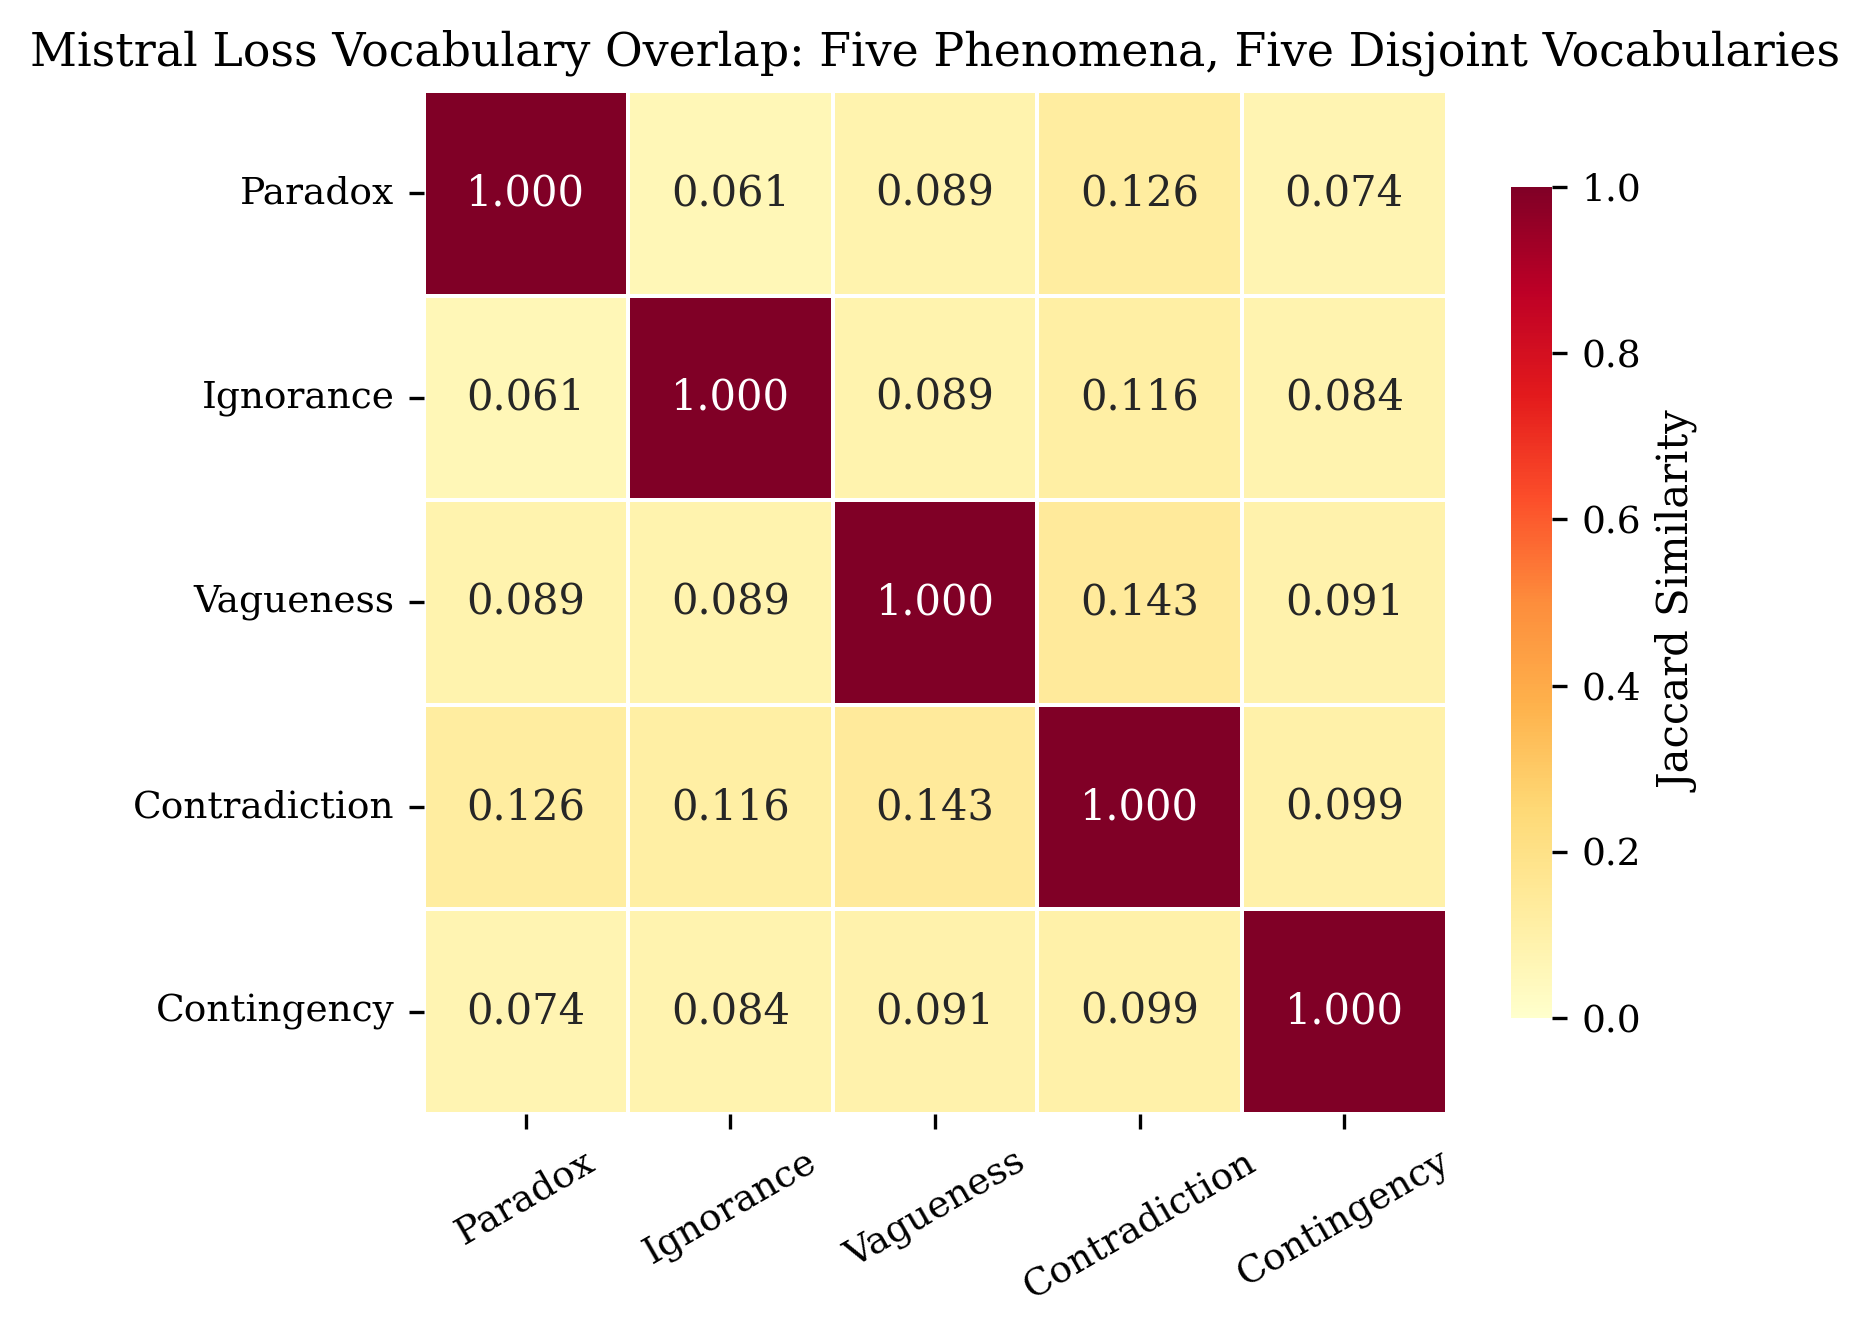
\includegraphics{fig_jaccard_heatmap.png}
\caption{Figure 3: Mistral pairwise Jaccard heatmap}
\end{figure}

\emph{Figure 3: Pairwise Jaccard similarity of Mistral's loss
vocabularies across all five phenomena. The hot diagonal
(self-similarity = 1.0) against uniformly cold off-diagonal cells (all
< 0.15) shows five nearly disjoint loss vocabularies from a
model that produces near-identical scalars.}

\subsection{Severity Profiles Add Further Discrimination}

Mean loss severity varies by phenomenon, even when scalars do not:

\begin{longtable}[]{@{}lcc@{}}
\toprule\noalign{}
Phenomenon & Mean Severity & Avg Losses/Rep \\
\midrule\noalign{}
\endhead
\bottomrule\noalign{}
\endlastfoot
Paradox & 0.795 & 4.2 \\
Contingency & 0.779 & 5.2 \\
Ignorance & 0.760 & 5.0 \\
Contradiction & 0.748 & 5.0 \\
Vagueness & 0.510 & 5.2 \\
\end{longtable}

Vagueness has markedly lower severity (0.510 vs 0.748--0.795),
reflecting that fuzzy boundary uncertainty is less severe than paradox
or ignorance. This is an appropriate distinction that the scalar
representation completely misses.

\subsection{Validation: Instruction-Following vs.\ Epistemic Assessment}
\label{sec:validation}

An adversarial reading of S4 might dismiss the results as ``just
instruction-following'': given a prompt that requests T/I/F values and
loss declarations, models dutifully produce both, and the apparent
structure is an artifact of compliance rather than evidence of internal
epistemic assessment.  We test this interpretation with four analyses
of the existing S4 data and two new experiments (72 additional API
calls).

\subsubsection{Test 1: Severity--Indeterminacy Correlation}

Across all 125 S4 evaluations, the maximum declared loss severity per
response correlates strongly with the corresponding I value: Pearson
$r = 0.78$ ($p < 10^{-26}$), Spearman $\rho = 0.83$
($p < 10^{-32}$).  The relationship holds within each of the five
models individually (all $p < 0.001$).  The S4 prompt requests T, I, F
values and loss declarations as independent output fields---it does not
instruct models to make severity correlate with indeterminacy.  Yet all
five models produce this internal coherence unprompted.

The mean--max distinction matters.  Mean severity shows a moderate
correlation ($r = 0.43$), but this is explained by stimulus identity:
harder stimuli produce both higher mean severity and higher~I.  After
residualizing by stimulus, the mean severity correlation disappears
($r = 0.02$, $p = 0.81$).  We report this honestly: the mean
severity relationship is a stimulus-level confound, not a within-cell
regularity.  Max severity, by contrast, survives stimulus
residualization ($r = 0.54$, $p < 10^{-10}$) and double
residualization removing both stimulus \emph{and} model effects
($r = 0.29$, $p < 0.001$).  The severity--indeterminacy coupling is
a within-cell structural relationship that cannot be attributed to
stimulus difficulty or model-level intercept differences.

\subsubsection{Test 2: Cross-Model Theme Convergence}

If loss declarations were templated compliance, different models would
produce either identical boilerplate or uncorrelated noise.  Instead, we
observe structured convergence: 8 epistemic themes achieved universal
agreement across all 5 models (mean pairwise Jaccard similarity 0.450;
permutation test $p < 0.0001$ for non-random convergence).

Theme content is stimulus-specific.  The liar paradox elicits
self-reference and bivalence-limits.  Rain elicits temporal uncertainty
and empirical-access limitations.  Stars elicits scope and
measurement-precision concerns.  Across all models and repetitions, the
S4 data contain 324 unique loss descriptions out of 417 total
declarations, with pairwise Jaccard similarity of exactly 0.000 between
all 10 stimulus pairs: not a single loss description appears in more
than one stimulus.

Models differ in depth but not direction.  Claude and Mistral produce
expansive declarations (4--6 losses per response); Llama and DeepSeek
produce efficient ones (2--3 losses).  All converge on the same themes
per stimulus.  This is stimulus-specific content generation with
cross-model structural agreement, not templated output.

\subsubsection{Test 3: Tautology Control}
\label{sec:tautology}

If models merely comply with format, they should produce similar I
values and severity scores for tautologies as for genuinely uncertain
stimuli---the prompt makes the same requests either way.  We tested
three tautologies:

\begin{enumerate}
\def\labelenumi{\arabic{enumi}.}
\tightlist
\item
  ``2+2=4'' (mathematical)
\item
  ``All bachelors are unmarried'' (definitional)
\item
  ``It is raining or it is not raining'' (logical)
\end{enumerate}

\noindent
across three models (Claude Sonnet 4.6, DeepSeek V3, Llama~4 Maverick),
3 repetitions each (27 API calls total).  Table~\ref{tab:tautology}
shows the comparison.

\begin{table}[t]
\centering
\caption{S4 responses for tautologies vs.\ original stimuli. Values are
means across all models and repetitions.}
\label{tab:tautology}
\begin{tabular}{lccccc}
\toprule
& \textbf{I} & \textbf{Max Severity} & \textbf{Mean Severity} & \textbf{Losses/Rep} \\
\midrule
Original stimuli ($n=125$)  & 0.739 & 0.740 & --- & 3.0 \\
Tautologies ($n=27$)        & 0.031 & 0.101 & --- & 2.0 \\
\midrule
\textbf{Ratio (taut/orig)}  & \textbf{0.04$\times$} & \textbf{0.14$\times$} & --- & 0.67$\times$ \\
\bottomrule
\end{tabular}
\end{table}

Indeterminacy drops by 25$\times$ and maximum severity by 7$\times$.
Loss count, however, drops only modestly (3.0 to 2.0): models comply
with the format requirement of declaring at least one loss but
\emph{modulate the content}.  Tautology losses are minimal-severity
hedges (``language ambiguity,'' ``formal system assumptions''), not the
substantive epistemic limitations declared for the original stimuli.

Two model-specific behaviors are instructive.  Claude refused $T = 1.0$
for any tautology, retaining a sliver of I (e.g., $I = 0.05$
for ``2+2=4'').  DeepSeek collapsed to exactly one loss at minimum
severity.  The logical tautology (``raining or not raining'') produced
slightly higher I values than the mathematical one---appropriate, since
excluded middle has genuine philosophical challenges that ``2+2=4'' does
not.\footnote{Tautology data: \texttt{data/tautology\_s4\_results.json}.}

\subsubsection{Test 4: Prompt Ablation}
\label{sec:ablation}

Tests 1--3 show that S4 responses are internally coherent and
content-modulated.  But they leave open the question of whether the
neutrosophic framing \emph{elicits} the epistemic assessment or merely
\emph{channels} it.  To test this, we stripped all neutrosophic
apparatus and ran a minimal prompt (S5):

\begin{quote}
\emph{``Identify any limitations, uncertainties, or difficulties in
determining whether this statement is true or false.''}
\end{quote}

\noindent
No T/I/F, no severity scores, no ``MUST declare losses.''  Same 5
stimuli, same 3 models, 3 repetitions each (45 API calls).
Table~\ref{tab:ablation} shows theme overlap between the S5 free-form
responses and the 10 reference themes identified in S4.

\begin{table}[t]
\centering
\caption{S5 (ablated prompt) theme overlap with S4 reference themes.
$\checkmark$ = theme present in all 3 repetitions;
\textsuperscript{$\circ$} = present in 2/3.
All 10 S4 reference themes appear in every model.}
\label{tab:ablation}
\begin{tabular}{lccc}
\toprule
\textbf{S4 Reference Theme} & \textbf{Claude} & \textbf{DeepSeek} & \textbf{Llama} \\
\midrule
Self-reference           & $\checkmark$ & $\checkmark$ & $\checkmark$ \\
Bivalence limits         & $\checkmark$ & $\checkmark$ & $\checkmark$ \\
Temporal uncertainty     & $\checkmark$ & $\checkmark$ & $\checkmark$ \\
Empirical access         & $\checkmark$ & $\checkmark$ & $\checkmark$ \\
Scope/cardinality        & $\checkmark$ & $\checkmark$ & $\checkmark$ \\
Measurement precision    & $\checkmark$ & $\checkmark$ & $\checkmark$ \\
Cultural norms           & $\checkmark$ & $\checkmark$ & $\checkmark$ \\
Contextual definitions   & $\checkmark$ & $\checkmark$ & $\checkmark$ \\
Moral pluralism          & $\checkmark$ & $\checkmark$ & $\checkmark$ \\
Consequentialist tension & $\checkmark$ & $\checkmark$ & $\checkmark$ \\
\bottomrule
\end{tabular}
\end{table}

The result is 100\% theme overlap: all 10 S4 reference themes appeared
in every model, every repetition, under the ablated prompt.  The
neutrosophic framing is not required to elicit the epistemic content.

S5 also produced 6 additional themes absent from S4:
language-ambiguity (42\% of responses), pragmatic-truth (22\%),
observer-dependence, incompleteness, logical-framework-choice, and
temporal-change.  Crucially, these are not evaluation-relevant losses
but \emph{task-preconditions}---observations about the difficulty of
evaluating rather than factors that affect the evaluation scores.
Language-ambiguity in ``it will rain tomorrow'' is real, but once one
has fixed the meanings of ``rain'' and ``tomorrow,'' the T/I/F
assessment proceeds without it.  The 6 extra themes describe conditions
that must be resolved \emph{before} evaluation begins, not uncertainty
that persists \emph{within} it.  Their absence from S4 output is
evidence that the formalism is working as intended: constraining the
observation space to what is relevant to the T/I/F
assessment.\footnote{Ablation data: \texttt{data/s5\_ablation\_results.json}.}

\subsubsection{Scope Confirmation}

The ablation reveals that S4 is a \emph{channel}, not a
\emph{source}.  The epistemic assessment pre-exists the prompt format;
S4 quantifies and standardizes it.  The 6 additional themes S5
surfaces are epistemically interesting but fall outside S4's scope
\emph{by design}: they are meta-level observations about the evaluation
task itself (``language is ambiguous,'' ``logical frameworks differ''),
not products of performing the evaluation.  This is what formal models
do---they exclude the irrelevant.  The S5 ablation confirms that S4
captures 100\% of evaluation-relevant themes (the 10 shared themes)
while correctly excluding preconditions that do not bear on T/I/F
scores.

S4's value is quantification and cross-model comparability: it converts
qualitative assessment into comparable tensors across models and stimuli.
The ablation confirms the scope of that conversion rather than exposing
a gap in it.

\subsubsection{Summary of the Validation Battery}

S4 also compresses I-value variance by 3--38$\times$ relative to
S1--S3 (38$\times$ for epistemic ignorance: S4 variance 0.0029 vs.\
S1--S3 variance 0.1112).  Requiring loss declarations anchors the
scalar assessment rather than decorating it.  Table~\ref{tab:battery}
summarizes the four tests.

\begin{table}[t]
\centering
\caption{Validation battery summary. Each test addresses a different
facet of the instruction-following objection.}
\label{tab:battery}
\begin{tabular}{lp{5.2cm}l}
\toprule
\textbf{Test} & \textbf{Finding} & \textbf{Against} \\
\midrule
Severity--I correlation & $r = 0.29$ after double residualization ($p < 0.001$)
  & Uncoupled compliance \\
Theme convergence & 8 universal themes, Jaccard = 0.000 cross-stimulus
  & Templated output \\
Tautology control & I drops 25$\times$, severity 7$\times$
  & Format-driven inflation \\
Prompt ablation & 100\% theme overlap; 6 extra precondition themes correctly outside S4 scope
  & Framing-dependent elicitation \\
\bottomrule
\end{tabular}
\end{table}

A compliant-but-uncoupled response to the S4 prompt would produce loss
severity uncorrelated with I (the prompt does not request coherence),
generic loss descriptions reused across stimuli (the prompt does not
prohibit this), unmodulated output for tautologies (the prompt makes
identical requests), and content dependent on neutrosophic framing (a
different prompt would elicit different themes).  The data show none of
these.  S4 surfaces pre-existing epistemic assessment; the neutrosophic
tensor structures it for comparison while correctly scoping to
evaluation-relevant factors.
